% \documentclass[12pt]{article}
% \usepackage[text={7.1 in, 8 in}, top=1.75in, left=0.69in]{geometry}
% \usepackage[round]{natbib}
% \usepackage[utf8]{inputenc}
% \usepackage{fullpage}
% \usepackage {setspace}
% \usepackage[hang,flushmargin]{footmisc} %control footnote indent
% \usepackage{url} % for website links
% \usepackage{amssymb,amsmath}%for matrix
% \usepackage{graphicx}%for figure
% \usepackage{appendix}%for appendix
% \usepackage{float}
% \floatstyle{plaintop}
% \restylefloat{table}
% \usepackage{multirow}
% \usepackage{longtable}
% \usepackage{morefloats}%in case there are too many float tables and figures
% \usepackage{caption}
% % \usepackage{subcaption}
% \usepackage{subfig}
% \captionsetup[subtable]{font=normal}
% \usepackage{hyperref}
% \usepackage{courier}
% \usepackage{color}
% \usepackage{setspace}
% \usepackage{rotating} % rotate table by some degree
% \usepackage{rotfloat}
% \usepackage{mwe}
% \usepackage{listings}
% \usepackage{titling}
% \usepackage{lipsum}
% \usepackage[export]{adjustbox}




% \graphicspath{{figures/}}

% \begin{document}
% \author{\small{\bf Ming Yang, Sheng Luo,
% and Stacia M. DeSantis}\\
% \small{Department of Biostatistics, The University of Texas Health Science Center at Houston}}
% \date{}
% \title{\large{\bf Web-based Supplementary Material for ``Model Estimation and Dynamic Prediction in Joint Modeling Using Longitudinal Quantile Regression''}}
% \maketitle{}


\subsection*{Appendices}
\addcontentsline{toc}{subsection}{Appendices}
\renewcommand{\thesubsubsection}{\Alph{subsubsection}}

\subsubsection{Distribution Comparison}

\begin{itemize}
\item Laplace distribution (LD) with location at 0 and scale parameter equals 1 is symmetrical about 0. It has heavier tail compared with standard normal distribution.
\item Asymmetric Laplace distribution (ALD) is either positively or negatively skewed and the direction and degree of skewness are control by the skewness parameter $\tau \in [0,1]$.
\end{itemize}

\begin{figure}[H]
\centering
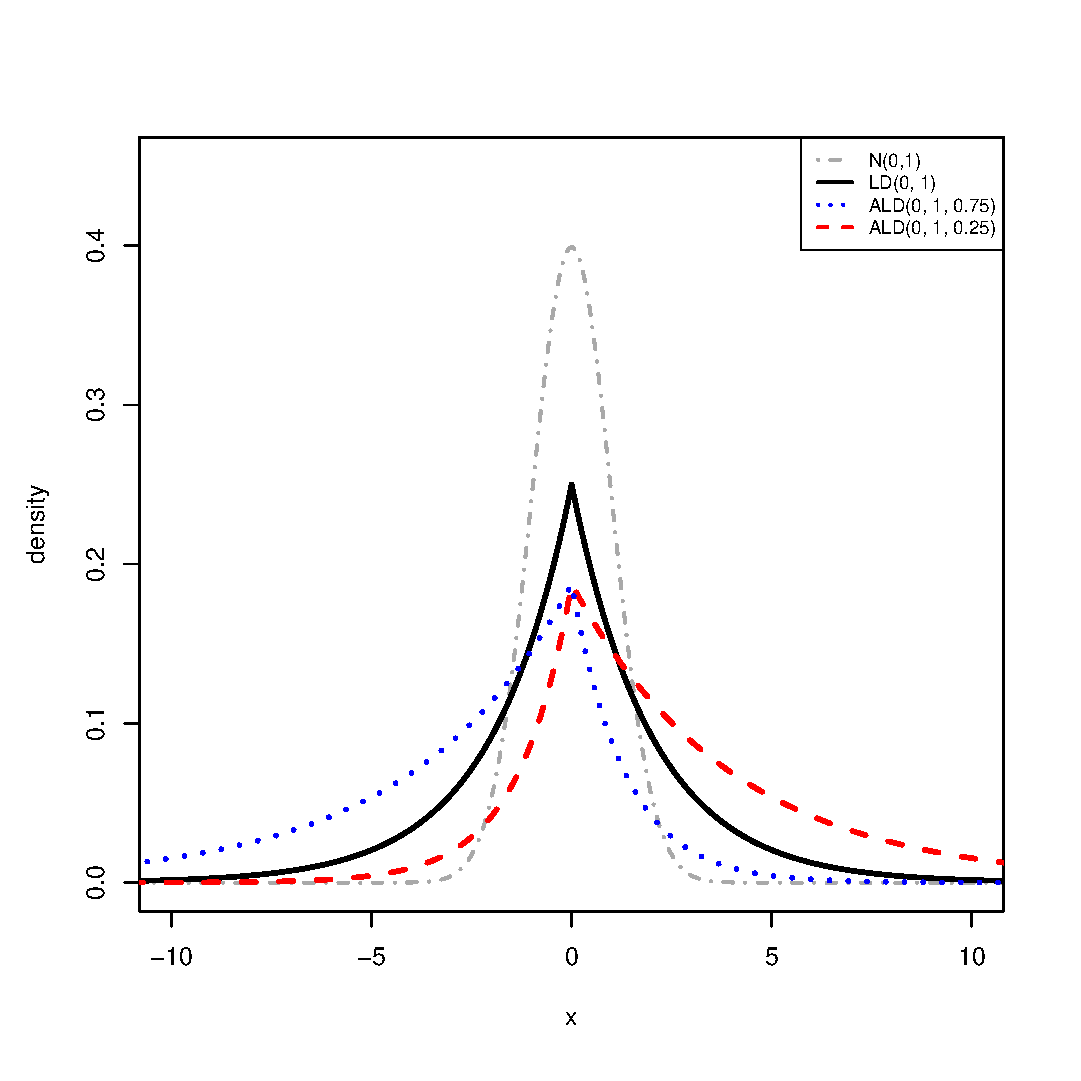
\includegraphics[width=0.6\columnwidth]{ald_ld_normal.eps}\label{plot:ald_ld_normal}
\caption{A comparison of normal, Laplace and asymmetric Laplace distributions.}
\end{figure}



\newpage
\subsubsection{Additional Simulation Results}\label{sec:appendix_simulation}

\begin{table}[H]
\centering
\caption{Simulation result in Simulation study I Scenario 2 in which random errors are generated from ALD with $\tau=0.5$.}
\adjustbox{max width=\textwidth}{
\label{tab:sim1tab2}
\begin{tabular}{lccccccccc}
\hline
& \multicolumn{4}{c}{QRJM ($\tau=0.5$)} & & \multicolumn{4}{c}{LMJM}\\
\hline
 & Bias & SE & MSE & CP & & Bias & SE & MSE & CP \\
\hline
  \multicolumn{10}{l}{Coefficients for longitudinal process} \\
  $\beta_0$ & $-$0.006 & 0.069 & 0.009 & 0.960 & & 0.013 & 0.093 & 0.017 & 0.960 \\
  $\beta_{1}$ & 0.008 & 0.060 & 0.008 & 0.900 & & 0.018 & 0.079 & 0.018 & 0.880 \\
  $\beta_{2}$ & 0.014 & 0.075 & 0.011 & 0.950 & & 0.031 & 0.093 & 0.021 & 0.940 \\
  \multicolumn{10}{l}{Coefficients for survival process} \\  
  $\gamma_1$ & 0.008 & 0.055 & 0.006 & 0.940 & & 0.014 & 0.058 & 0.007 & 0.950 \\
  $\gamma_2$ & 0.007 & 0.055 & 0.007 & 0.950 & & 0.013 & 0.057 & 0.007 & 0.950 \\
  $\alpha$ & $-$0.001 & 0.071 & 0.011 & 0.930 & & $-$0.028 & 0.101 & 0.086 & 0.920 \\
   \hline
\end{tabular}
}
\end{table}


% latex table generated in R 3.2.2 by xtable 1.7-4 package
% Tue Oct 27 23:07:31 2015
\begin{table}[H]
\centering
\caption{Simulation result in Simulation study I Scenario 3 in which random errors are generated from $\mathcal{N}(0, 1)$.}
\adjustbox{max width=\textwidth}{
\label{tab:sim1tab3}
\begin{tabular}{lccccccccc}
\hline
& \multicolumn{4}{c}{QRJM ($\tau=0.5$)} & & \multicolumn{4}{c}{LMJM} \\
\hline
 & Bias & SE & MSE & CP & & Bias & SE & MSE & CP \\
\hline
  \multicolumn{10}{l}{Coefficients for longitudinal process} \\

  $\beta_0$ & 0.015 & 0.037 & 0.003 & 0.950 & & 0.000 & 0.035 & 0.002 & 0.980 \\
  $\beta_{1}$ & 0.004 & 0.034 & 0.002 & 0.960 & & $-$0.003 & 0.033 & 0.002 & 0.950\\
  $\beta_{2}$ & 0.013 & 0.050 & 0.005 & 0.950 & & 0.006 & 0.049 & 0.005 & 0.950 \\
  \multicolumn{10}{l}{Coefficients for survival process} \\  
  $\gamma_1$ & 0.008 & 0.055 & 0.006 & 0.920 & & 0.003 & 0.054 & 0.006 & 0.900 \\
  $\gamma_2$ & 0.015 & 0.055 & 0.007 & 0.920 & & 0.010 & 0.054 & 0.006 & 0.920 \\
  $\alpha$ & $-$0.013 & 0.055 & 0.006 & 0.950 & & 0.007 & 0.055 & 0.006 & 0.950 \\
   \hline
\end{tabular}
}
\end{table}


\begin{table}[H]
\centering
\caption{Prediction results in Simulation study II Scenario 3 in which random errors are generated from ALD with $\tau=0.5$.}
\adjustbox{max width=\textwidth}{
\label{tab:sim2tab2}
\begin{tabular}{clccccc}
\hline
 & & \multicolumn{2}{c}{QRJM ($\tau=0.5$)} & &\multicolumn{2}{c}{LMJM}\\
\cline{3-4}\cline{6-7}
$t$ & $\Delta t$ & MSE & Bias & & MSE & Bias \\
\hline
\multirow{2}{*}{{\bf 0.25}} & 0.25 & 0.005 & 0.005 && 0.005 & $-$0.001 \\
&  1 & 0.009 & 0.005 &&  0.009 & 0.000 \\
\multirow{2}{*}{(subjects left: 47.87\%)} &  2 & 0.011 & 0.003 && 0.010 & 0.000 \\
&  3 & 0.011 & 0.002 && 0.011 & 0.001 \\
\hline
\multirow{2}{*}{{\bf 0.5}} & 0.25 & 0.004 & 0.005 && 0.003 & $-$0.002 \\
&   1 & 0.009 & 0.004 && 0.008 & $-$0.002 \\
\multirow{2}{*}{(subjects left: 34.78\%)}&   2 & 0.012 & 0.002 && 0.011 & $-$0.001 \\
&   3 & 0.013 & 0.001 && 0.012 & $-$0.001 \\
\hline
\multirow{2}{*}{{\bf 0.75}} & 0.25 & 0.002 & 0.004 && 0.002 & $-$0.002 \\
& 1 & 0.009 & 0.005 && 0.007 & $-$0.002 \\
\multirow{2}{*}{(subjects left: 27.71\%)} & 2 & 0.012 & 0.002 && 0.011 & $-$0.003 \\
&  3 & 0.014 & 0.001 && 0.012 & $-$0.002 \\
\hline
\end{tabular}
}
\end{table}


\begin{figure}[H]
\centering
\subfloat[][QRJM with $\tau=0.25$ (True model)]{
    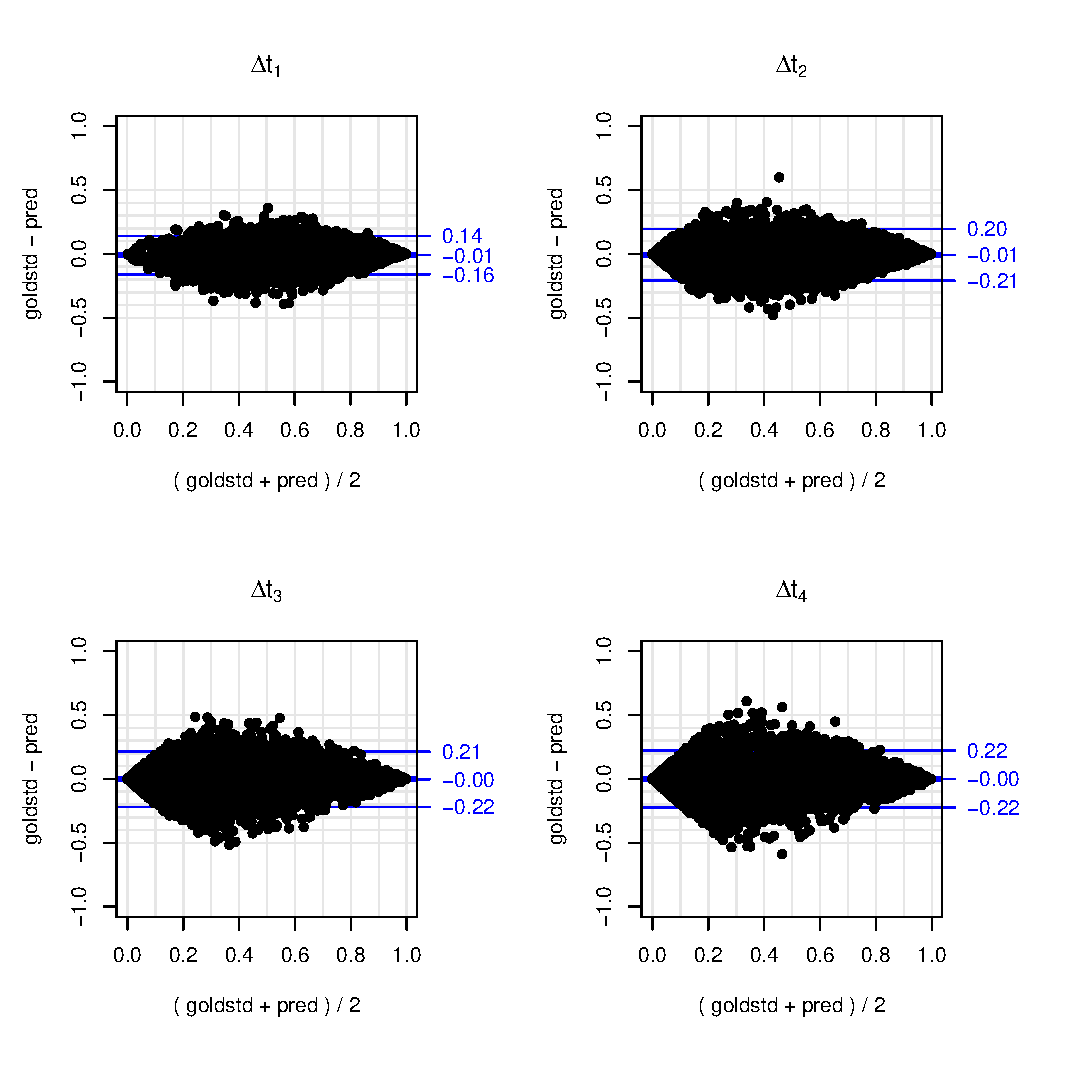
\includegraphics[width=0.45\columnwidth]{baplot_qt25data_qt25fit_t1.eps}\label{plot:sim2fig11}
}
% \centering
\subfloat[][QRJM with $\tau=0.5$]{
    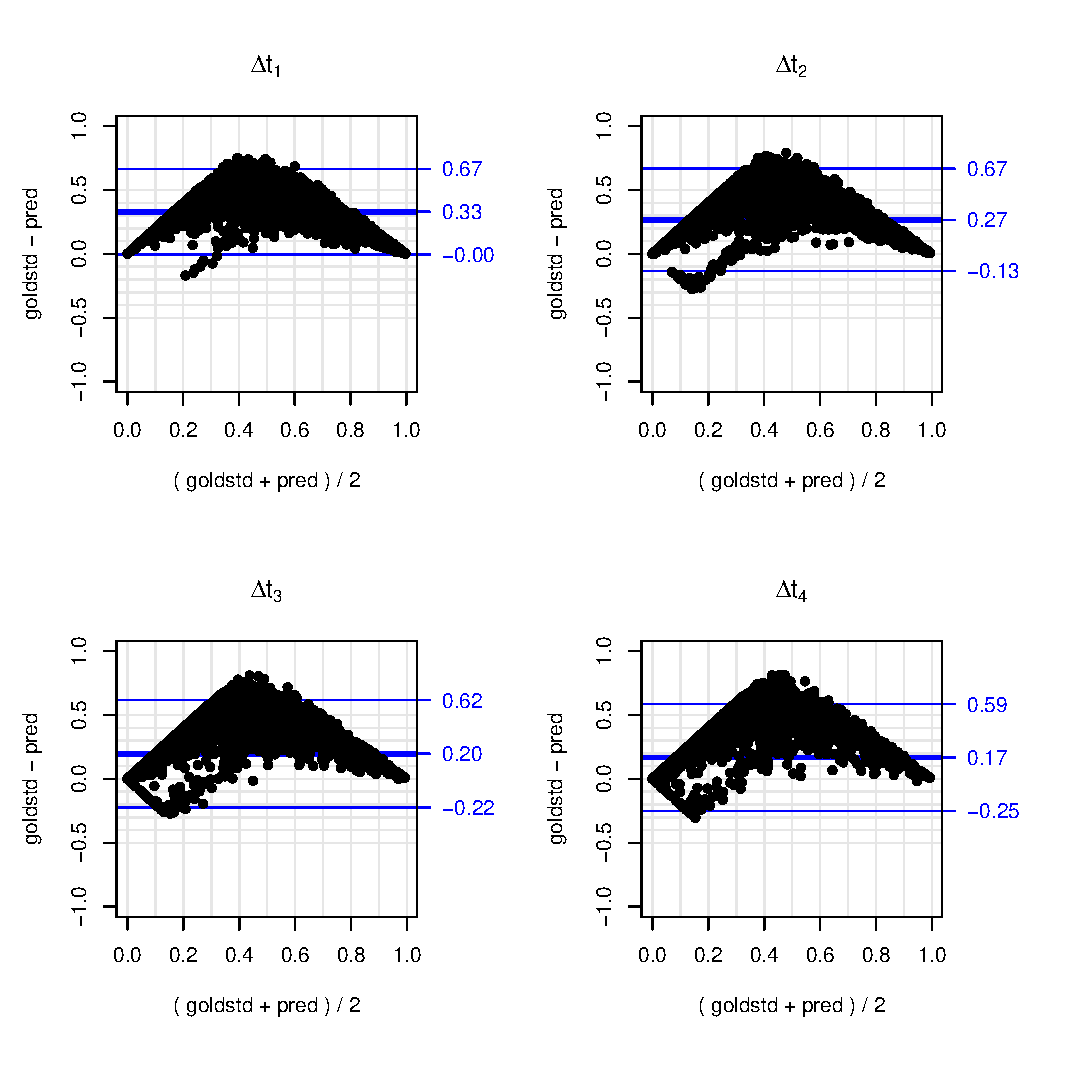
\includegraphics[width=0.45\columnwidth]{baplot_qt25data_qt50fit_t1.eps}\label{plot:sim2fig12}
}

\subfloat[][LMJM]{
    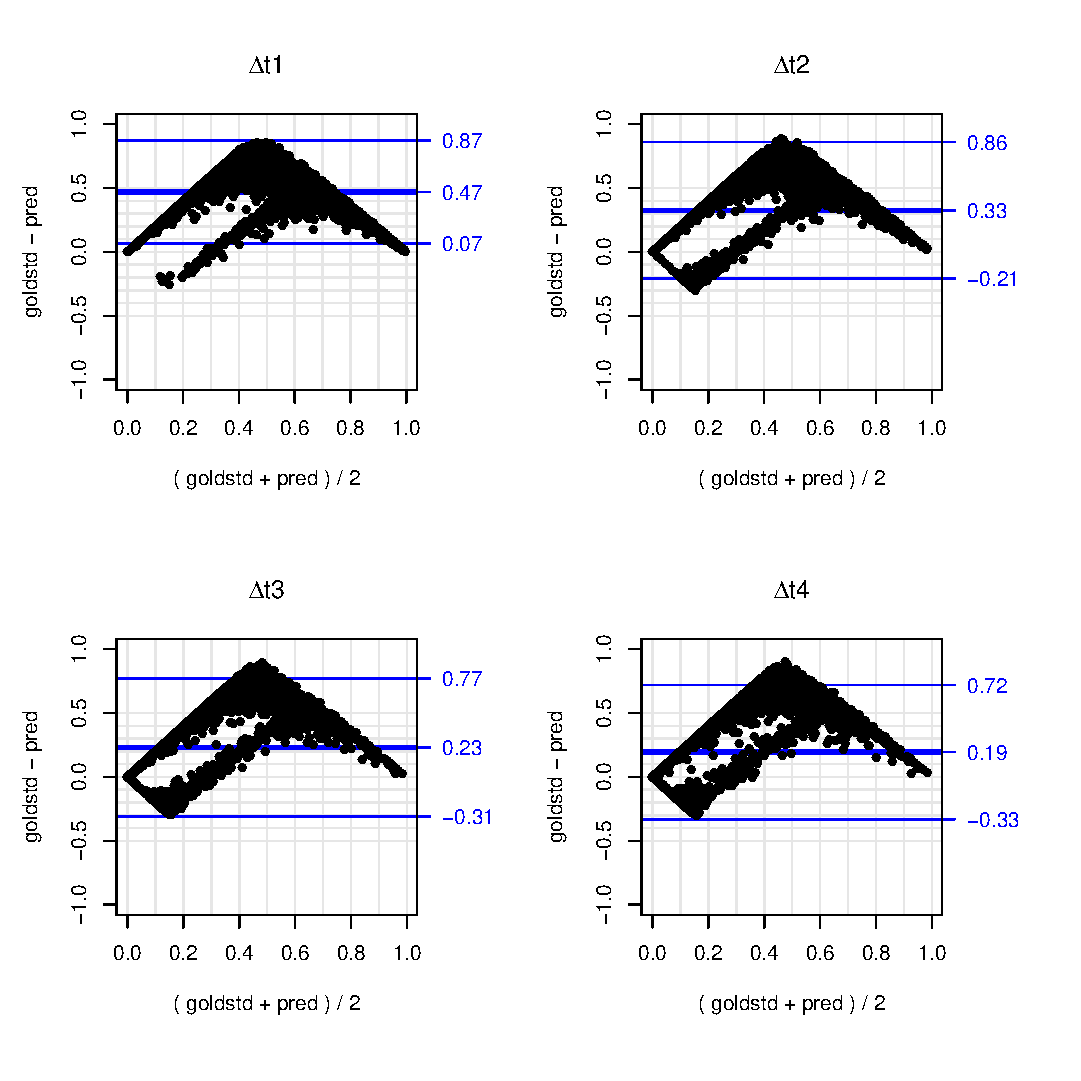
\includegraphics[width=0.45\columnwidth]{baplot_qt25data_LMJMfit_t1.eps}\label{plot:sim2fig13}
}
  \caption{Prediction results in Simulation study II Scenario 1: Bland-Altman plot (bias and 95\% limits of agreement) of gold standard versus model predictions at four prediction time intervals ($\Delta t_1 < \Delta t_2 < \Delta t_3 < \Delta t_4$).}
  \label{plot:sim2fig1}
\end{figure}

\begin{figure}[H]
\centering
\subfloat[][LMJM (True model)]{
    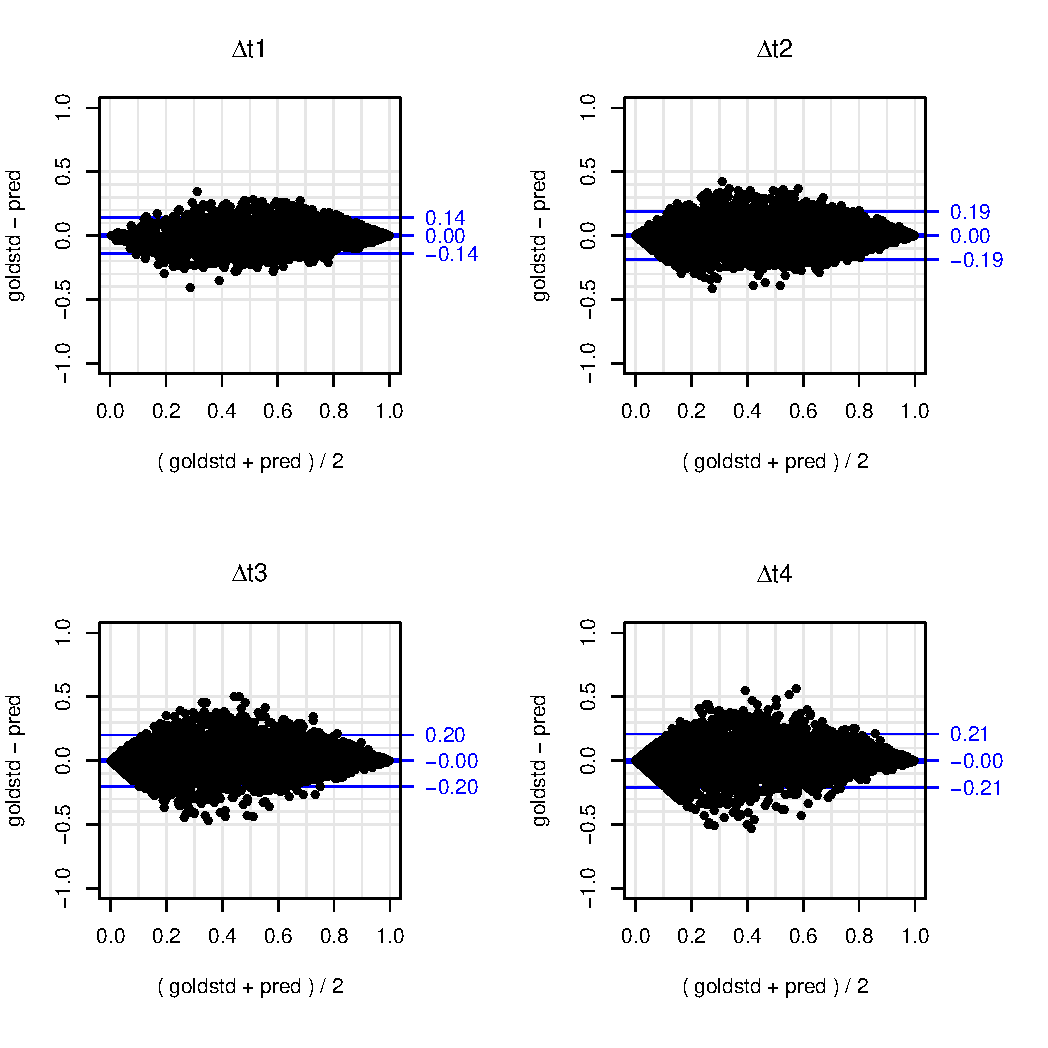
\includegraphics[width=0.45\columnwidth]{baplot_normdata_LMJMfit_arms_t1.pdf}\label{fig:3a}
}
% \centering
\subfloat[][QRJM with $\tau=0.5$]{
    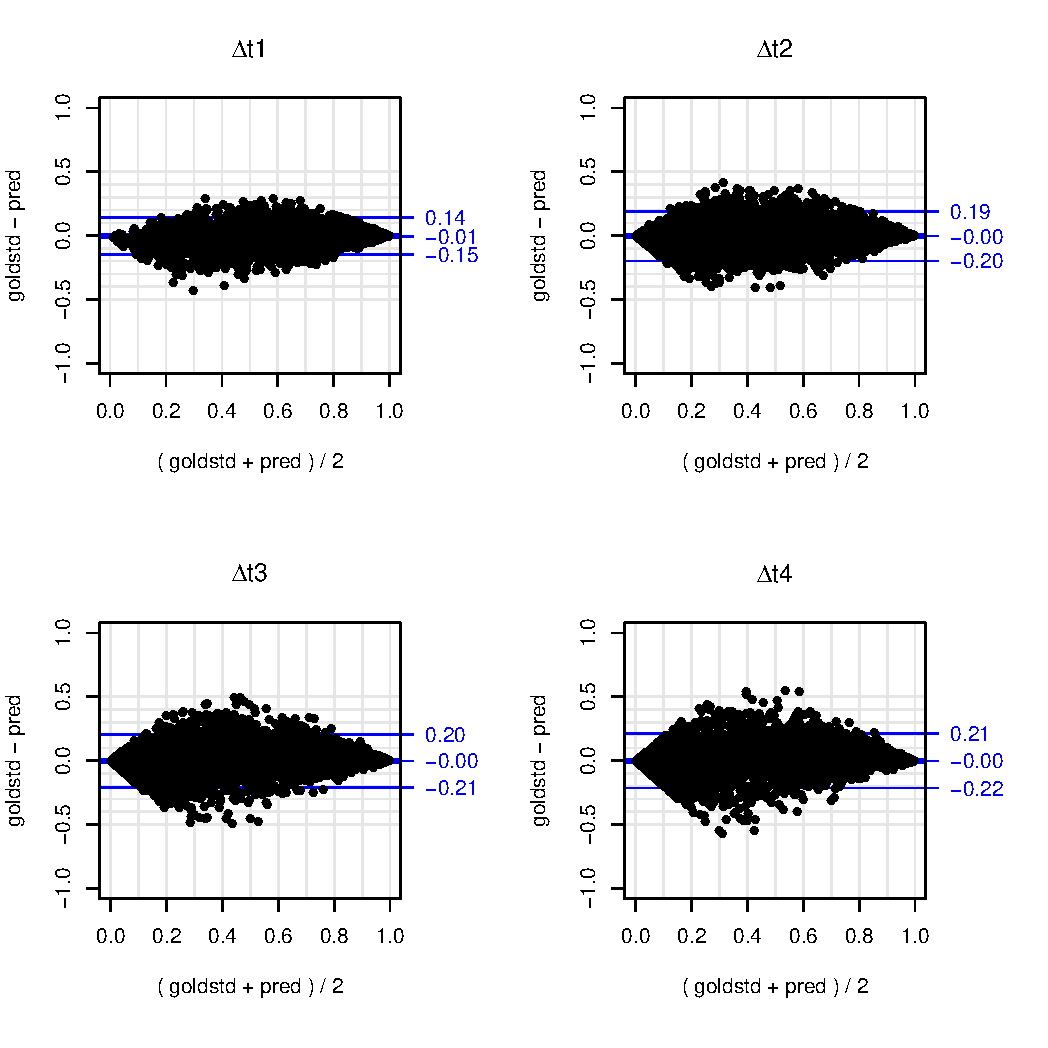
\includegraphics[width=0.45\columnwidth]{baplot_normdata_qt50fit_arms_t1.pdf}\label{fig:3b}
}
  \caption{Prediction results in Simulation study II Scenario 3: Bland-Altman plot (bias and 95\% limits of agreement) of gold standard versus model predictions based on the first two longitudinal observations and four different prediction time intervals ($\Delta t_1 < \Delta t_2 < \Delta t_3 < \Delta t_4$).}
  \label{plot:sim2fig2}
\end{figure}



\subsubsection{Variable Definitions}\label{sec:appendix_var_description}
\begin{itemize}
\item {Total motor score}: Standardized ratings of oculomotor function, dysarthria, chorea, dystonia, gait and postural stability based on the Unified Huntington Disease Rating Scale (UHDRS).

\item {Putamen}: the volume of putamen, which a round structure located at the base of the forebrain. The atrophy of the putamen is related with impaired movements regulation and learning ability.

\item {Stroop word}: Stroop Color and Word Test score. The test consists of three 45-second trials, including two trials measure basic attention and process speed and a third trail tests the ability to identifying the name of a color (e.g., ``blue'', ``green'', or ``red'') that is printed in a color not denoted by the name.

\item {FrBe executive subscale}: Frontal System Behavioral Scale -- executive subscale -- companion rating scale. Part of a 46-item behavior rating scale on abstraction, problem solving, and hypothesis generation as rated by a companion focusing on dorsolateral prefrontal circuitry.

\item {Total functional capacity}: A list of independent and common daily tasks that can be accomplished bas on the UHDRS.

\end{itemize}



\subsubsection{LOESS Plots of Selected Longitudinal Variables}

\begin{figure}[H]
\centering
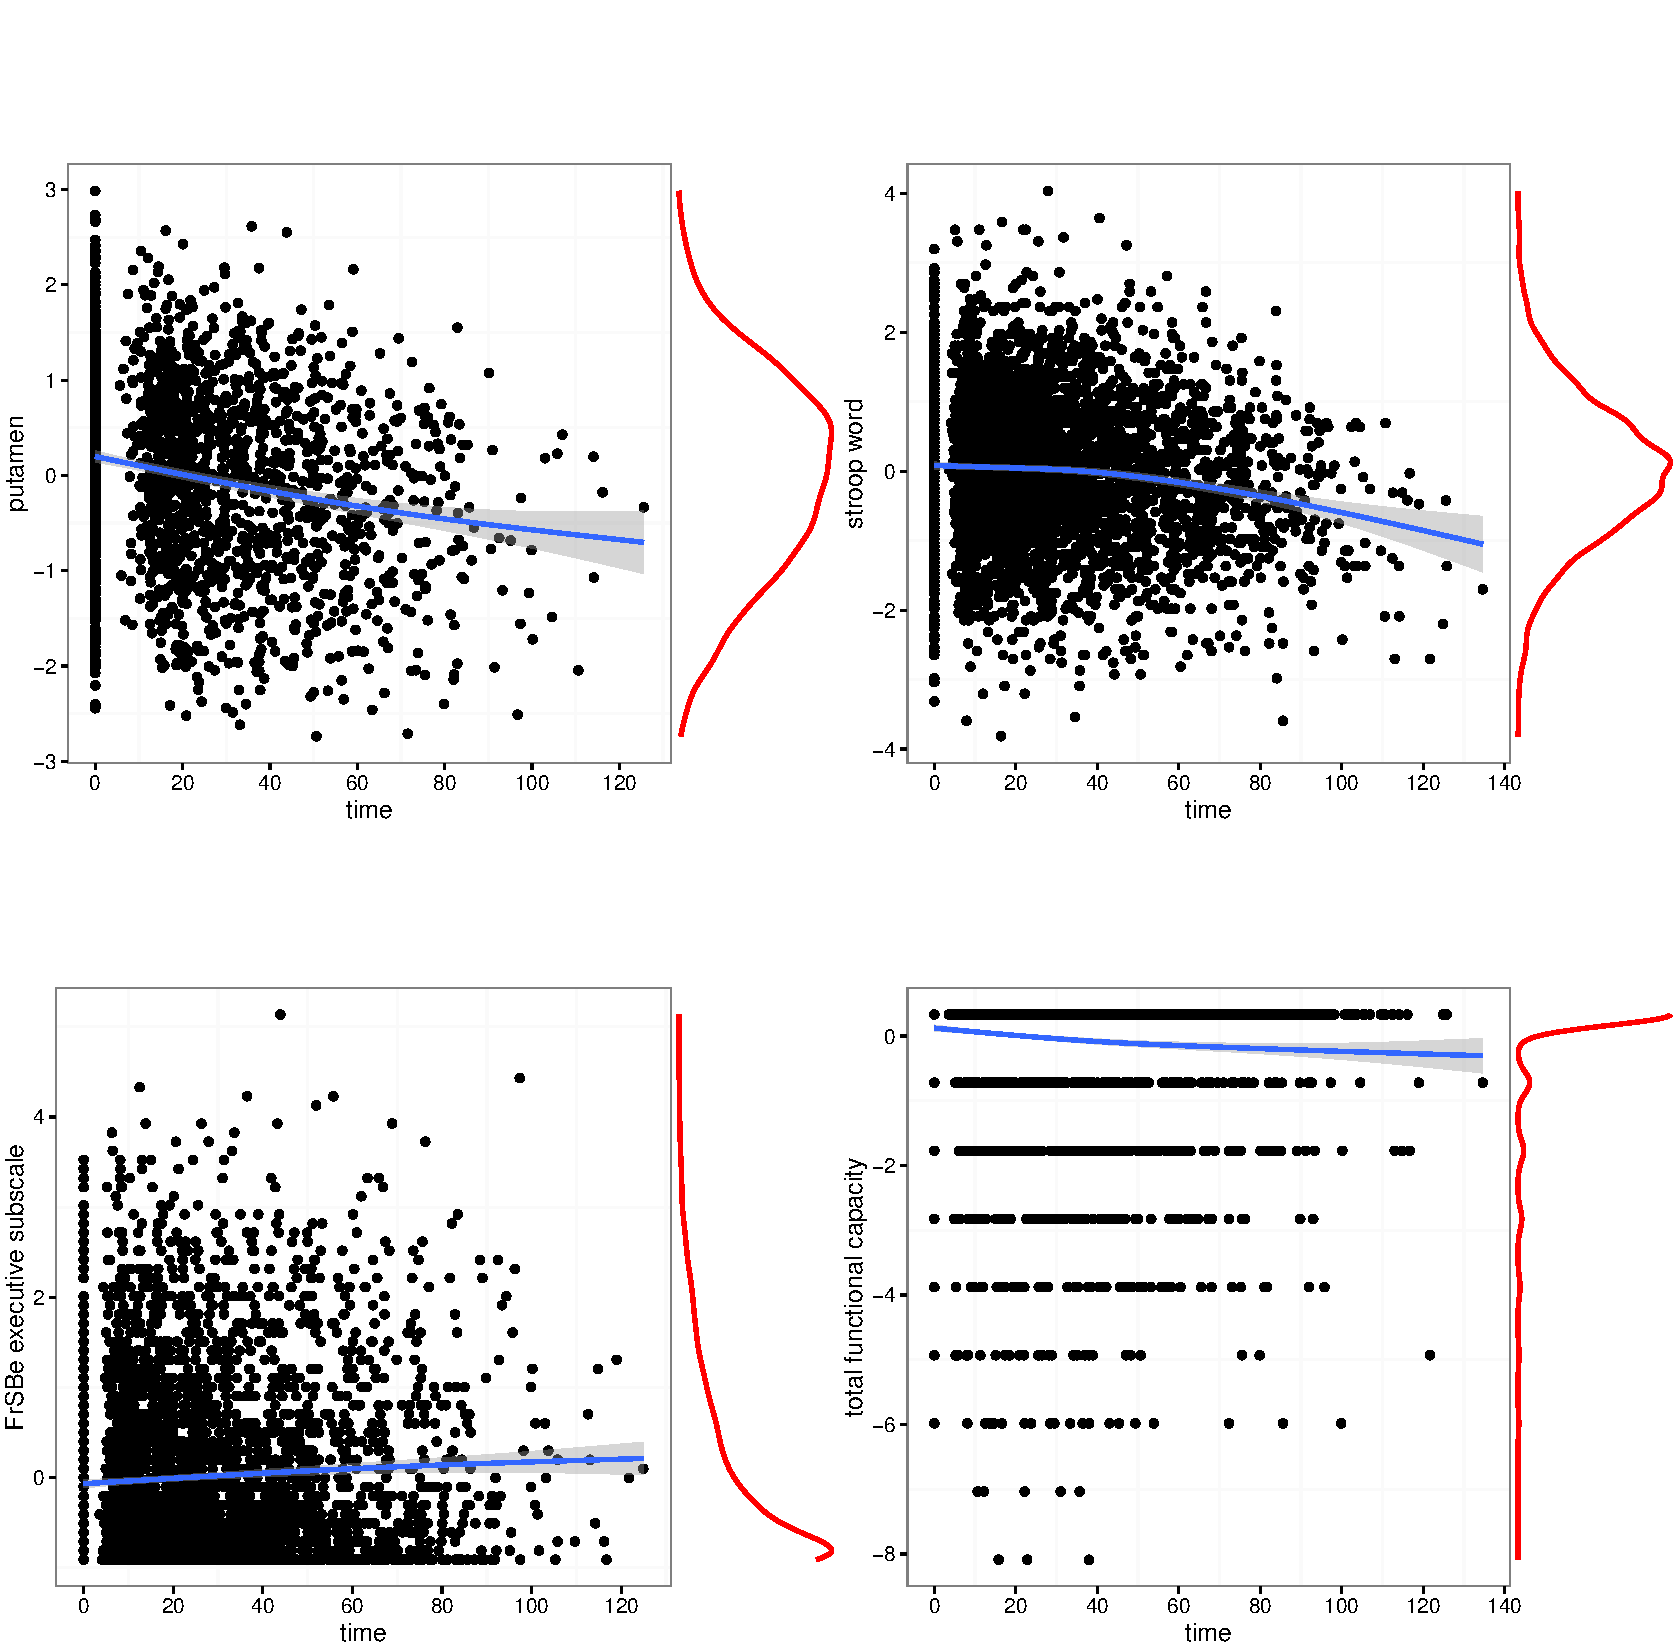
\includegraphics[width=1.0\linewidth]{data_densities_loess.pdf}
\caption{Scatter plot with LOESS curve for {putamen (top left)}, {stroop word (top right)}, {FrBe executive subscale (bottom left)} and {total functional capacity (bottom right)} from the study population.}
\label{fig:data_densities}
\end{figure}

\singlespacing
\section{Additional Data Analysis Results}\label{sec:appendix_realdata}
\begin{table}[H]
\centering
\caption{PREDICT-HD data analysis: Parameter estimation and 95\% credible interval (in parenthesis) from QRJM at three quantiles (0.25, 0.5, and 0.75) with putamen, stroop word, FrBe executive subscale (FES), and total functional capacity (TFC) being the longitudinal biomarkers.}
\label{realdata_inference}
\resizebox{\linewidth}{!}{
\begin{tabular}{l ccc r ccc}
  \hline
  & \multicolumn{3}{c}{{putamen}}&& \multicolumn{3}{c}{{stroop word}}\\
  \hline
  & $\tau=0.25$ & $\tau=0.50$ & $\tau=0.75$ & & $\tau=0.25$ & $\tau=0.50$ & $\tau=0.75$\\
\hline
\multicolumn{8}{l}{For longitudinal process} \\
int. & 1.045 & 1.142  & 0.1.243 && 0.123  & 0.370 & 0.625 \\
  &(0.830, 1.266)& (0.864, 1.439) & (1.003, 1.511) && (-0.136, 0.378) & (0.114, 0.640) & (0.382, 0.857) \\

time (month) & -0.014 & -0.014  & -0.014 && -0.007 & -0.007 & -0.007\\
  & (-0.018, -0.010) & (-0.017, -0.010) & (-0.017, -0.010) && (-0.010, -0.004) & (-0.010, -0.003) & (-0.010, -0.004)\\

$age_0$ & -0.023 & -0.023  & -0.017 && -0.006 & -0.007 & -0.007 \\
  & (-0.028, -0.018) & (-0.030, -0.017) & (-0.029, -0.017) && (-0.013, 0.000) & (-0.013, 0.000) & (-0.013, -0.001)\\ \\

\multicolumn{8}{l}{For time to HD onset process} \\
assoct. & -1.038 & -1.039  & -1.045 && -0.696 & -0.709 & -0.719 \\
  & (-1.213, -0.861)& (-1.217, -0.860) & (-1.224, -0.862) && (-0.832, -0.558) & (-0.846, -0.573) & (-0.853, -0.581) \\

eduyr & -0.060 & -0.055  &  -0.050 && -0.080 & -0.069 & -0.059  \\
  & (-0.094, -0.027)& (-0.093, -0.021) & (-0.090, -0.015) && (-0.106, -0.053) & (-0.097, -0.043) & (-0.088, -0.032)\\

male & -0.021 & -0.020 & -0.017 && -0.173 & -0.166 & -0.157 \\
  & (-0.347, 0.283)& (-0.336, 0.290) & (-0.330, 0.303) && (-0.459, 0.111) & (-0.458, 0.111) & (-0.449, 0.124) \\
  \hline
  \hline
  & \multicolumn{3}{c}{{FrBe executive subscale}}&& \multicolumn{3}{c}{{total functional capacity}}\\
  \hline
  & $\tau=0.25$ & $\tau=0.50$ & $\tau=0.75$ & & $\tau=0.25$ & $\tau=0.50$ & $\tau=0.75$ \\
\hline
\multicolumn{8}{l}{For longitudinal process}\\
int. & -0.533 & -0.244 & 0.138 && 0.277  & 0.333 & 0.362  \\
  & (-0.731, -0.328) & (-0.493, -0.021) & (0.261, 0.494) && (0.218, 0.355) & (0.293, 0.372) &  (0.330, 0.394)\\

time (month) & 0.007 & 0.006 & 0.006 && -0.028 & -0.016 & -0.007 \\
  & (0.003, 0.011) & (0.003, 0.010) & (0.002, 0.010) && (-0.033, -0.024) & (-0.020, -0.012) &  (-0.012, -0.004)\\

$age_0$ & 0.002 & 0.002 & 0.001 && -0.001  & -0.000 & 0.000 \\
  & (-0.003, 0.007) & (-0.003, 0.008) & (-0.006, 0.008) && (-0.002, 0.001) & (-0.001, -0.001) &  (-0.001, 0.001)\\\\

\multicolumn{8}{l}{For time to HD onset process}\\
assoct. &  0.524 & 0.434 & 0.376 && -0.374 & -0.478 &  -0.488\\
  & (0.378, 0.667) & (0.306, 0.435) & (0.261, 0.494) && (-0.438,-0.305) & (-0.569, -0.389) &  (-0.596, -0.378)\\

eduyr & -0.077 & -0.082 & -0.091 && -0.097 & -0.093 &  -0.093 \\
  & (-0.116, -0.041) & (-0.119, -0.052) & (-0.125, -0.060) && (-0.135, -0.064) & (-0.134, -0.058) &  (-0.138, -0.054) \\

male & -0.263 & -0.301 & -0.291 && 0.104 & 0.057 & 0.031 \\
  & (-0.560, 0.051) & (-0.611, 0.004) & (-0.602, 0.006) && (-0.207, 0.405) & (-0.260, 0.354) &  (-0.286, 0.329) \\
  \hline
\end{tabular}
}
\end{table}


\doublespacing
\newpage
\subsubsection{\textsf{JAGS} Model File}\label{p1:jags_code}
\textsf{JAGS} model file to fit QRJM in simulation study.
{\scriptsize
\begin{verbatim}
model{
      k1 <- (1-2*qt)/(qt*(1-qt))
      k2 <- 2/(qt*(1-qt))
      for (i in 1:I){
        # prior for random effects
        u[i, 1:2] ~ dmnorm(zero[], precision[,])
        # longitudinal process
        for (j in 1:J[i]){
            er[i,j] ~ dexp(sigma)
            mu[i,j] <- beta + u[i,1] + u[i,2]*t[j] + time[1]*X[i,1]
                    + time[2]*X[i,2]*t[j] + k1*er[i,j]
            prec[i,j] <- sigma/(k2*er[i,j])
            y[i,j] ~ dnorm(mu[i,j], prec[i,j])
        } #end of j loop
        # time-to-event process
        A[i] <- assoct.*u[i,2] + assoct.*time[2]*X[i,2]
        B[i] <- assoct.*(time[1]*X[i,1] + u[i,1] + beta) + inprod(gamma, W[i,])
        S[i] <- exp(-c*exp(B[i])*(exp(A[i]*Ti[i])-1)/A[i])
        h[i] <- c*exp(inprod(gamma, W[i,]) + assoct.*(beta +
            time[1]*X[i,1] + time[2]*X[i,2]*Ti[i] + u[i,1] + u[i,2]*Ti[i]))
        L[i] <- pow(h[i], event[i])*S[i]/1E+08
        phi[i] <- -log(L[i])
        zeros[i] ~ dpois(phi[i])
    }#end of i loop
    precision[1:2, 1:2] ~ dwish(Omega[,], 3)
    Sigma[1:2,1:2] <- inverse(precision[,])
    Omega[1,1] <- 1
    Omega[2,2] <- 1
    Omega[1,2] <- 0
    Omega[2,1] <- 0
    # priors for other parameters
    assoct. ~ dnorm(0, 0.001)
    int. ~ dnorm(0, 0.001)
    time[1] ~ dnorm(0, 0.001)
    time[2] ~ dnorm(0, 0.001)
    gamma[1] ~ dnorm(0, 0.001)
    gamma[2] ~ dnorm(0, 0.001)
    sigma ~ dgamma(0.001, 0.001)
    c ~ dunif(0.01, 10)
}
\end{verbatim}
}
